%====================================================================
%====================================================================
\section{Combining variational inference with ...}
\frame{\frametitle{Outline} \tableofcontents[currentsection]}
%====================================================================
\subsection{Frequentist inference}
%====================================================================
\frame{\frametitle{Frequentist inference} \pause

  \paragraph{Maximum likelihood inference.}
  $$
  \widehat{\theta}_{MLE} = \argmax_\theta \; \log p_\theta(Y)
  $$
  is intractable because the likelihood involves an integration over the latent $Z$
  \begin{align*}
  \text{PLN:} \qquad 
  \log p_\theta(Y) & = \sum_i \log \left(\emphase{\int_{\Rbb^p}} p_\Sigma(Z_i) \prod_j p_\beta(Y_{ij} \mid Z_{ij}) \d Z_i \right) \\
  ~ \\
  \text{SBM:} \qquad 
  \log p_\theta(Y) & = \log \left(\emphase{\sum_{Z \in [K]^n}} \prod_i p_\pi(Z_i) \prod_{i, j} p_{\alpha, \beta}(Y_{ij} \mid Z_i, Z_j) \right) 
  \end{align*}
  
  \pause \bigskip \bigskip
  The (log-)likelihood is far from being the only admissible estimation function \\
  ~ \\
  \ra think, e.g., of $M$-estimation

}
  
%====================================================================
\frame{\frametitle{Composite likelihood} 

  \paragraph{Sum of partial likelihoods:} 
  \begin{align*}
  \text{PLN:} \qquad 
  \widehat{\theta}_{CL} 
  & = \argmax_\theta \; \sum_i \sum_{j, k} \log p_\theta(Y_{ij}, Y_{ik}) &
  & \text{only requires $\int_{\Rbb^2}$} \\
  ~ \\
  \text{SBM:} \qquad 
  \widehat{\theta}_{CL} 
  & = \argmax_\theta \; \sum_{i, j, k} \log p_\theta(Y_{ij}, Y_{ik}, Y_{jk}) &
  & \text{only requires $\sum_{Z \in [K]^3}$} \\
  \end{align*}
  \ra Generic results (consistency, asymptotic normality) exist for $\widehat{\theta}_{CL}$ \refer{VRF11} +  see \refer{AmM12} for binary SBM
  
  \pause \bigskip \bigskip 
  \paragraph{Practical implementation.}
  \begin{itemize}
  \item EM algorithms can be designed to maximize composite likelihoods
  \item \bigskip Getting $\widehat{\theta}_{CL}$ is still demanding (many terms in the sum: $np^2$ for PLN, $n^3$ for SBM)
  \item \bigskip $\widehat{\theta}_{VEM}$ usually provides a (very) good starting point
  \end{itemize}


}
  
%====================================================================
\subsection{Bayesian inference}
%====================================================================
\frame{\frametitle{Bayesian inference} \pause

  \paragraph{Reminder.}
  \begin{itemize}
  \item Prior: $p(\theta)$ \qquad \qquad \qquad \textcolor{gray}{$\theta_{PLN} = (\beta, \Sigma)$, \quad $\theta_{SBM} = (\pi, \alpha, \beta)$}
  \item Latent: $p(Z \mid \theta)$
  \item Observed: $p(Y \mid Z, \theta)$
  \item Posterior:
  $$
  p(\theta, Z \mid Y) = \frac{p(\theta) \; p(Z \mid \theta) \; p(Y \mid, \theta, Z)}{p(Y)}
  $$
  \end{itemize}

  \pause \bigskip 
  \paragraph{Sampling methods.}
  \begin{itemize}
  \item \pause Monte-Carlo: sample $(\theta^b, Z^b) \overset{\text{iid}}{\sim} p(\theta, Z \mid Y)$
  \item \pause MCMC: construct a Markov chain with $p(\theta, Z \mid Y)$ as a stationary distribution
  \item \pause Importance sampling: $(\theta^b, Z^b) \overset{\text{iid}}{\sim} q(\theta, Z )$ and reweight each draw with weight
  $$
  w^b = \frac{p(\theta^b, Z^b \mid Y)}{q(\theta^b, Z^b)}
  $$
  \item \pause Sequential Monte-Carlo: construct a sequence of distribution going from $q(\theta, Z )$ to $p(\theta, Z \mid Y)$
  \end{itemize}

}

%====================================================================
\frame{\frametitle{Sequential Monte-Carlo sampling} 

  \begin{tabular}{cc}
    \hspace{-.04\textwidth}
    \begin{tabular}{p{.5\textwidth}} 
      \paragraph{Principle.} \refer{DDJ06} $U = (\theta, Z)$ \\ ~ 
      \begin{itemize}
        \item \pause given $\textcolor{blue}{p_{{start}}(U)}$ \\ ~ 
        \item \pause aiming at $\textcolor{red}{p_{{target}}(U)} =  p(U \mid Y)$ \\ ~
        \item \pause sample from a sequence of distributions
%         $p_{\text{start}} = p_0$, $p_1$, $\dots$, $p_{H-1}$, $p_H = p_{\text{target}}$
        $$
        \textcolor{blue}{p_{{start}} = p_0}, \; p_1, \; \dots, \; p_{H-1}, \; \textcolor{red}{p_H = p_{{target}}}
        $$
        with
        $$
        p_h(U) \propto p_{{start}}(U)^{{1 - \rho_h}} p_{{target}}(U)^{{\rho_h}}
        $$
        and $0 = \rho_0 < \rho_1 \ < \dots < \rho_H = 1$
      \end{itemize}
    \end{tabular}
    &
    \begin{tabular}{p{.45\textwidth}}
      \includegraphics[width=.4\textwidth]{\figbayes/FigVBEM-IS-Tempering-4to2} \\
      \textcolor{gray}{see \#\ref{goto:SMC} for tuning of the $\rho_h$} \label{back:SMC}
    \end{tabular}
  \end{tabular}
  
  \pause \bigskip 
  \begin{description}
  \item[Most often:] $p_{{start}} = p_{prior}$ \qquad (long way to the posterior)
  \item[VBEM:] \smallskip directly use $p_{{start}} = p_{VBEM}$
  \item[VEM:] \smallskip use (approximate) Louis formulas \refer{Lou82} to derive $p_{{start}} = p_{VEM}$ \refer{DoR19}
  \end{description}

  
} 

%====================================================================
\frame{\frametitle{Back to the tree interaction network} 

  \begin{tabular}{ccc}
    \hspace{-.04\textwidth}
    \begin{tabular}{p{.35\textwidth}}
      $$
      \begin{array}{rl}
      Y_{ij} & = \text{number of shared parasites} \\
      x_{ij} & = \text{taxonomic distance} \\
      Y_{ij} & \sim \Pcal(\exp(x_{ij}^\intercal \beta + \alpha_{Z_iZ_j}))
      \end{array}
      $$
      ~ \\

      \paragraph{Estimates:}
      $$
      \widehat{K}_{ICL} = 4
      \qquad 
      \widehat{\beta} = -.317
      $$
      {\begin{itemize}
      \item Taxonomy (partially) explains the links (smaller $\widehat{K}$)
      \item \bigskip Distant species share less parasites ($\widehat{\beta} < 0$)
      \item \bigskip The remaining structure is \emphase{not related to taxonomy}
      \end{itemize}}
    \end{tabular}
    &
    \hspace{-.05\textwidth}
    \begin{tabular}{p{.3\textwidth}}
      \paragraph{No covariate:} $\widehat{K}_{ICL} = 7$ \\
      \includegraphics[height=.3\textwidth, width=.3\textwidth]{\fignet/Tree-adjMat-SBMnull} \\
      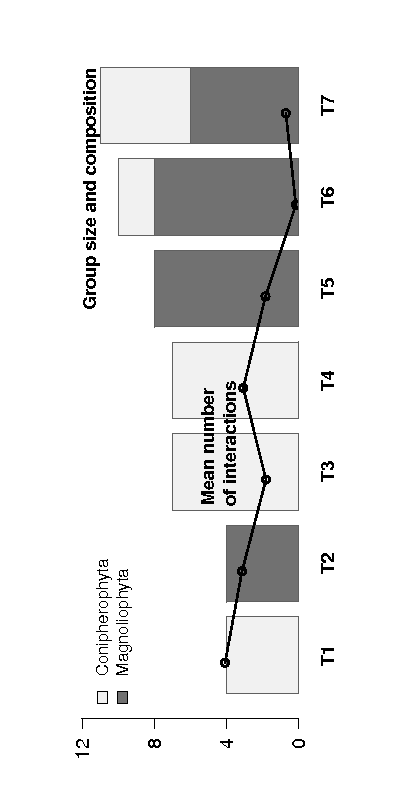
\includegraphics[height=.3\textwidth, width=.3\textwidth, trim=150 150 150 150]{\fignet/MRV10_AoAS_Q7_group}
    \end{tabular}
    &
    \hspace{-.05\textwidth}
    \begin{tabular}{p{.3\textwidth}}
      \paragraph{Taxonomic dist.:} $\widehat{K}_{ICL} = 4$ \\
      \includegraphics[height=.3\textwidth, width=.3\textwidth]{\fignet/Tree-adjMat-SBMtaxo} \\
      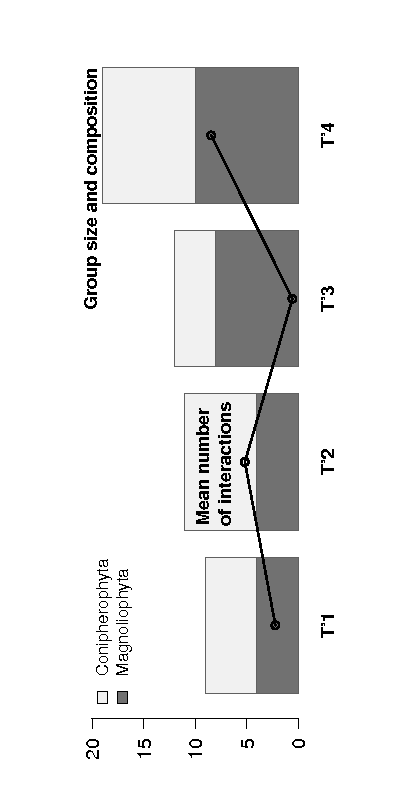
\includegraphics[height=.3\textwidth, width=.3\textwidth, trim=150 150 150 150]{\fignet/MRV10_AoAS_Q4_group}
    \end{tabular}
  \end{tabular}

}

%====================================================================
\frame{\frametitle{Tree network: model selection} 

  \paragraph{Model selection.} 
  \begin{itemize}
  \item Number of groups $K$ 
  \item Set $S$ of relevent covariates: $S \subset \{\text{taxonomy, geography, phylogeny}\}$
  \end{itemize}
  
  \pause \bigskip 
  \begin{tabular}{ccc}
    \hspace{-.04\textwidth}
    \begin{tabular}{p{.4\textwidth}}
      \paragraph{Choosing $K$} for a given $S$:
      $$
      p(K \mid Y, S) \propto p(Y \mid S, K)
      $$
      here : $S = (\text{taxonomy, geography})$ \\
      ~ \\ 
      \textcolor{gray}{Averaging over $K$: \#\ref{goto:graphon}} \label{back:graphon} \\
      ~ \\
    \end{tabular}
    &
    \begin{tabular}{p{.3\textwidth}}
      \includegraphics[width=.25\textwidth]{\figDoR/Tree-all-V10-M5000-logpY}
    \end{tabular}
    &
    \hspace{-.1\textwidth}
    \begin{tabular}{p{.2\textwidth}}
      $\log p(Y \mid S, K)$ \\ ~ \\
      \textcolor{blue}{$J_{\widehat{\theta}, \widehat{q}}$} \\ ~ \\
      \textcolor{red}{$vICL$} \\ 
    \end{tabular}
  \end{tabular}
  
  \pause \bigskip \bigskip 
  \paragraph{Variable selection.} $p(S \mid Y) = \sum_K p(S, K \mid Y)$
  $$
  P\{x = \text{(taxo., geo.)} \mid Y \} \simeq 70\%, \qquad
  P\{x = \text{(taxo.)} \mid Y \} \simeq 30\%
  $$

}

%====================================================================
\frame{\frametitle{Tree network: significance} 

  \paragraph{Parameter posterior distribution} for $S = (\text{taxonomy, geography, phylogeny})$: 
  $$
  \begin{array}{ccc}
    \text{taxonomy} & \text{geography} & \text{phylogeny} \\
    \includegraphics[width=.25\textwidth]{\figDoR/Tree-all-V10-M5000-beta1} & 
    \includegraphics[width=.25\textwidth]{\figDoR/Tree-all-V10-M5000-beta2} & 
    \includegraphics[width=.25\textwidth]{\figDoR/Tree-all-V10-M5000-beta3} \\
    \multicolumn{3}{l}{\text{Legend:} \qquad 
      \textcolor{blue}{q_{VEM}(\beta_j)}, \qquad 
      \textcolor{red}{p(\beta_j \mid S, \widehat{K}(S), Y)}, \qquad 
      p(\beta_j \mid S, Y) }
  \end{array}
  $$
  
  \bigskip \pause
  \paragraph{Why so many steps} to go from \textcolor{blue}{$q_{VEM}(\beta_j)$} to \textcolor{red}{$p(\beta_j \mid Y)$} ?
  
  \bigskip 
  \hspace{-.025\textwidth}
  \begin{tabular}{rrrr}
    \paragraph{Correlation between estimates.} 
    & $(\beta_1, \beta_2)$ & $(\beta_1, \beta_3)$ & $(\beta_2, \beta_3)$ \\
    $p_{VEM}(\beta)$    & $-0.012$ & $ 0.021$ & $ 0.318$ \\
    $p(\beta \mid Y)$ & $-0.274$ & $-0.079$ & $-0.088$
  \end{tabular}
  
  \bigskip
  \textcolor{gray}{+ $p(Z \mid Y)$ in \#\ref{goto:smcPath}} \label{back:smcPath}

}
